\documentclass[12pt]{article}
\usepackage{polski}
\usepackage[utf8]{inputenc}
\usepackage[margin=1in]{geometry}
\usepackage[polish]{babel}
\usepackage{graphicx}
\usepackage{indentfirst}
\usepackage{graphicx}
\usepackage{float}
\usepackage{textcomp}
\usepackage{caption}
\usepackage{listings}
\usepackage{color}
\usepackage{hyperref}
\usepackage{booktabs}
\usepackage{tabularx}
\usepackage{longtable}
\usepackage{array}
\usepackage[table,xcdraw]{xcolor}
% If you use beamer only pass "xcolor=table" option, i.e. \documentclass[xcolor=table]{beamer}

\lstset{language=Python,
	keywordstyle=\color{blue},
	stringstyle=\color{red},
	morecomment=[l][\color{magenta}]{\#},
	showspaces=false,
	showstringspaces=false,
	frame=single
}

\begin{document}
	
	\thispagestyle{empty}
	
	\begin{flushright}2 grudnia 2018\end{flushright}
	
	\noindent
	Piotr Cieszko 226079 \\
	Wojciech Ormaniec 226181 \\
	
	\vspace{1em}
	
	\noindent
	grupa: \\
	czwartek TP, $8^{15}$-$11^{00}$
	
	\vfill
	
	\begin{center}
		\begin{Large}
			Internetowe Bazy Danych
		\end{Large}
		
		\vspace{2cm}
		
		\begin{Huge}
			System wspierający działanie firmy w warstwie informacyjnej
			
		\end{Huge}
		
		\vspace{1cm}
		
		\begin{Large}
			
		\end{Large}
	\end{center}
	
	\vspace{3cm}
	
	\noindent
	\begin{Large}
		Prowadzący: \\
		\vspace{.5cm}
		\indent
		dr inż. Roman Ptak
	\end{Large}
	
	\vspace{1cm}
	
	\noindent
	\begin{Large}
		Rok akademicki: \\
		\vspace{.5cm}
		\indent
		2018/2019
	\end{Large}
	
	\vfill
	
	\newpage
	
	\tableofcontents
	
	\newpage
	
	\section{Założenia projektowe}
	
	Celem projektu jest stworzenie aplikacji internetowej, która będzie realizować określone funkcjonalności w firmie klienta z uwzględnieniem łatwości dalszej rozbudowy.
	
	Podstawą tej aplikacji będzie system zarządzania pracownikami oraz klientami firmy - zarządzanie dostępem, podstawowymi danymi personalnymi oraz udostępnionymi funkcjami.
	
	\begin{itemize}
		\item
		Pierwszą funkcjonalnością będzie zarządzanie fakturami, które wystawiamy klientom. Klient, któremu pracownik nadał dostęp do tych zasobów, może samodzielnie pobierać udostępnione faktury. Pracownicy z kolei mogą zarządzać fakturami w systemie, wraz z przypisaniem do określonego użytkownika.
		\item
		Drugą rzeczą do zaimplementowania jest system powiadomień. Klient może otrzymać powiadomienie wysłane przez pracownika do niego bądź do wszystkich klientów.
		\item
		Ostatnią będzie proste forum. Możliwość tworzenia wątków, udzielania się w nich, jeden poziom kategorii tematycznych. Notyfikacje o pojawieniu się nowych postów.
	\end{itemize}
	
	\subsection{Przypadki użycia}
	
	Wspólne przypadki użycia dla administratora, pracownika i klienta zostały oznaczone wspólną linią, pokolorowaną dodatkowo kolorem czerwonym dla czytelności.
	
	\begin{figure}[H]
		\centering
		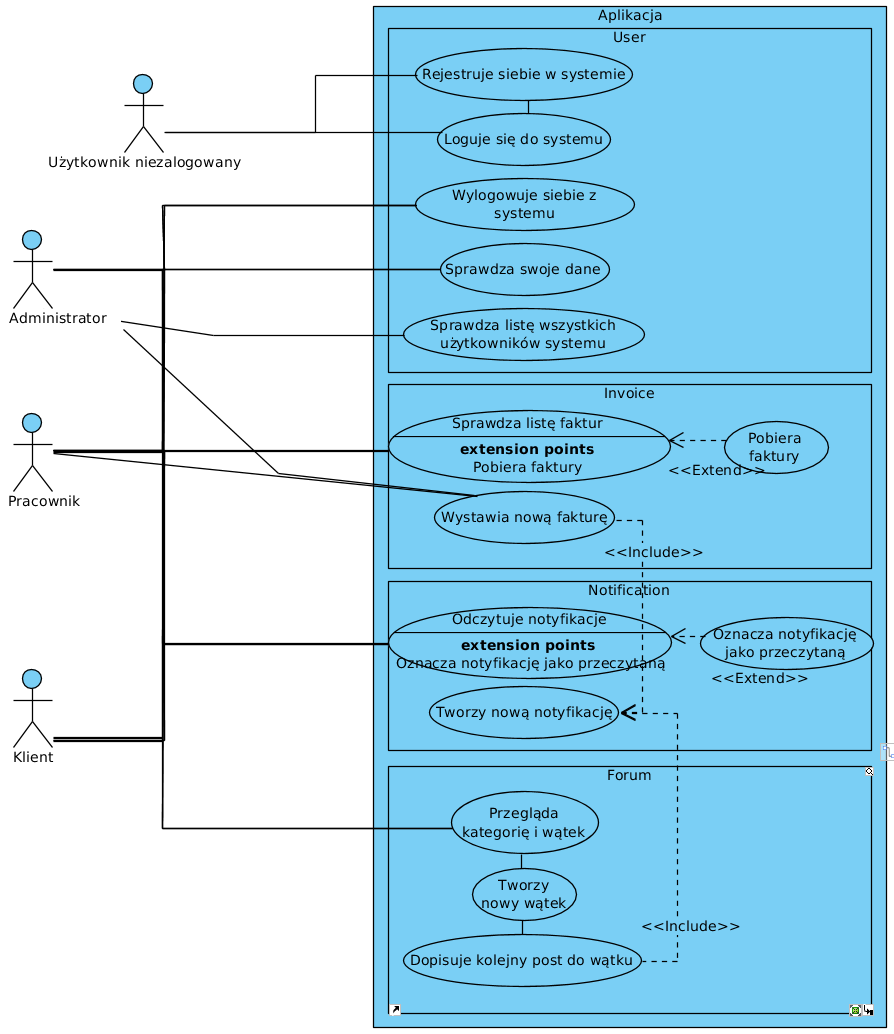
\includegraphics[scale=0.55]{img/przejscia.png}
		\caption{Diagram przypadków użycia}
		\label{}
	\end{figure}
	\newpage
	
	\subsection{Bezpieczeństwo}
	Strona będzie zabezpieczona przed nieuprawnionym dostępem poprzez system logowania. W przypadku dostępu do strony bez należytych uprawnień, zostanie wyświetlony komunikat o błędzie.
	
	\subsection{Przewidywane technologie}
	Po stronie klienta:
	\begin{itemize}
		\item HTML 5
	\end{itemize}
	Po stronie serwera:
	\begin{itemize}
		\item Linux
		\item Python
		\item Django
		\item SQLite
	\end{itemize}
	
	\section{Analiza SWOT}
	\begin{figure}[H]
		\centering
		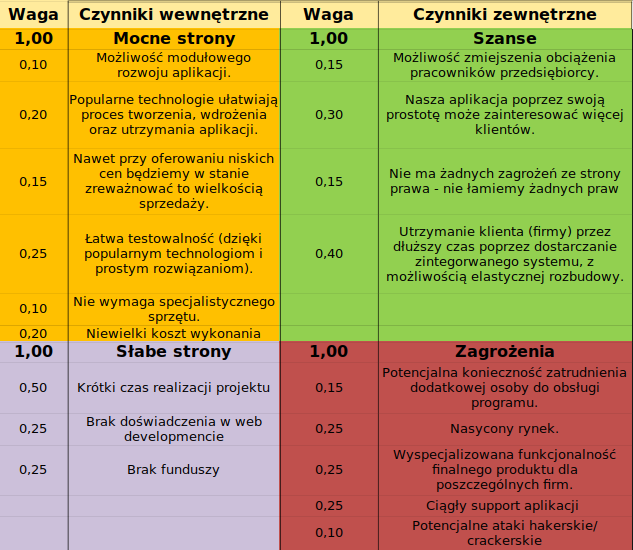
\includegraphics[scale=1.0]{img/swot1.png}
		\caption{Czynniki analizy SWOT}
	\end{figure}
	\subsection{Analiza powiązań SWOT}
	\begin{figure}[H]
		\centering
		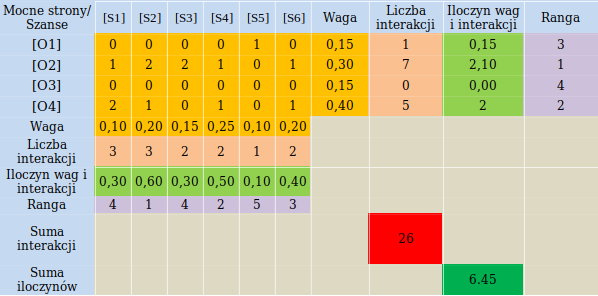
\includegraphics[scale=1.0]{img/swot2.png}
		\caption{Czy określona mocna strona pozwala wykorzystać daną szansę?}
	\end{figure}
	\begin{figure}[H]
		\centering
		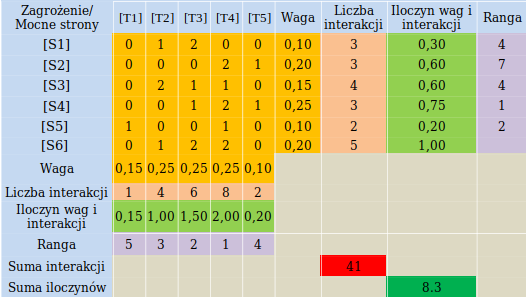
\includegraphics[scale=1.1]{img/swot3.png}
		\caption{Czy określona mocna strona pozwala ograniczyć dane zagrożenie?}
	\end{figure}
	\begin{figure}[H]
		\centering
		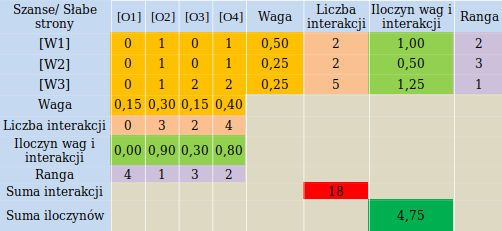
\includegraphics[scale=1.1]{img/swot4.png}
		\caption{Czy określona słaba strona ogranicza możliwość wykorzystania danej szansy?}
	\end{figure}
	\begin{figure}[H]
		\centering
		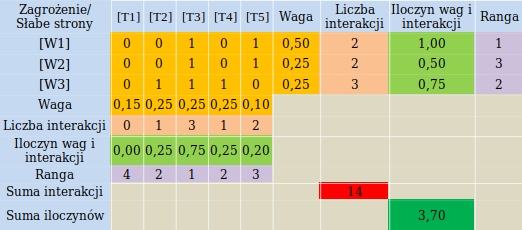
\includegraphics[scale=1.1]{img/swot5.png}
		\caption{Czy określona słaba strona potęguje dane zagrożenie?}
	\end{figure}
	
	Z przeprowadzonej analizy wynika, że korzystna będzie zarówno strategia konserwatywna (8.30), jak i agresywna (6.45).
	\newpage
	\section{Techniczna wykonalność projektu}
	Do wykonania projektu potrzebujemy:
	\begin{itemize}
		\item Czas i umiejętności potrzebne do:
		\begin{itemize}
			\item stworzenia aplikacji (programiści, projektanci, etc.)
			\item utrzymania wdrożenia u klienta
		\end{itemize}
		\item Sprzęt:
		\begin{itemize}
			\item komputery do tworzenia aplikacji
			\item serwer do hostowania aplikacji u klienta
		\end{itemize}
		\item Oprogramowanie:
		\begin{itemize}
			\item Python 3.6
			\item Django 2.1.2
			\item Baza danych (SQLite 3)
			\item System operacyjny (Linux)
			\item Przeglądarka internetowa (Firefox, inne)
			\item Środowisko programistyczne (PyCharm)
			
		\end{itemize}
	\end{itemize}
	
	\section{Kosztorys}
	\begin{itemize}
		\item Tworzenie aplikacji i wdrożenie: 60h * 40zł = 2400zł
		\item Utrzymanie wdrożenia u klienta (1 rok): 20h * 40zł = 800zł
		\item Komputery – prywatne (koszt amortyzacji): 40zł
		\item Serwer wirtualny (1 rok): 360zł (posiadający Python 3.6)
		\item Domena: 150zł
		\item Python: 0zł
		\item Django: 0zł
		\item SQLite: 0zł
		\item Linux: 0zł
		\item Firefox: 0zł
		\item PyCharm: 0zł
	\end{itemize}
	Suma (wykonanie + 1 rok utrzymania):\textbf{ 3750zł }
	\newpage
	\section{Instrukcja dla użytkownika}
	\subsection{Rejestracja w systemie}
	Po otworzeniu strony widzimy stronę główną.
	\begin{figure}[H]
		\centering
		
\includegraphics[scale=0.5]{img/1.png}
		\caption{Strona główna}
	\end{figure}
	Po wciśnięciu przycisku 'Register' przechodzimy do stosownego formularza.
	\begin{figure}[H]
		\centering
		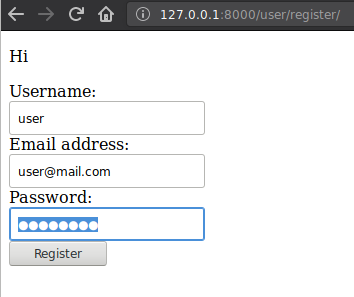
\includegraphics[scale=0.5]{img/2.png}
		\caption{Formularz rejestracji}
	\end{figure}
	Po wypełnieniu klikamy 'Register' i zostajemy automatycznie zalogowani na nasze nowe konto. W pierwszym wierszu widzimy nazwę naszego konta ('user').
	\begin{figure}[H]
		\centering
		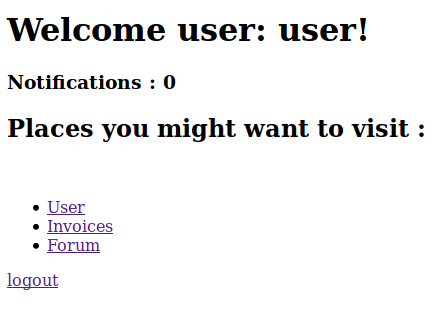
\includegraphics[scale=0.5]{img/3.png}
		\caption{Strona po zalogowaniu}
	\end{figure}
	
	\subsection{Logowanie do systemu}
	Na stronie głównej wybieramy przycisk 'Login'.
	\begin{figure}[H]
		\centering
		
\includegraphics[scale=0.5]{img/1.png}
		\caption{Strona główna}
	\end{figure}
	Po czym wprowadzamy nasze dane i zatwierdzamy.
	\begin{figure}[H]
		\centering
		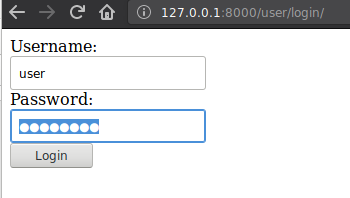
\includegraphics[scale=0.5]{img/4.png}
		\caption{Logowanie}
	\end{figure}
	
	\subsection{Wylogowanie z systemu}
	Aby się wylogować, naciskamy przycisk logout na stronie głównej.
	\begin{figure}[H]
		\centering
		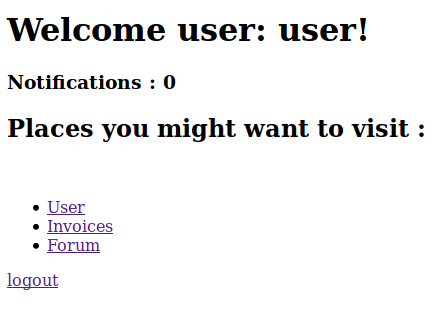
\includegraphics[scale=0.5]{img/3.png}
		\caption{Strona po zalogowaniu}
	\end{figure}
	\subsection{Sprawdzenie informacji o sobie}
	Na stronie głównej wybieramy 'User'.
	\begin{figure}[H]
		\centering
		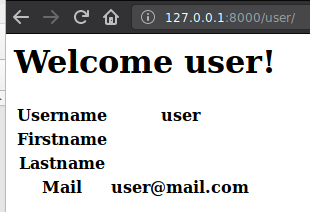
\includegraphics[scale=0.7]{img/5.png}
		\caption{Informacje o użytkowniku}
	\end{figure}
	\subsection{Odczytywanie notyfikacji}
	Gdy pojawi się nowy komunikat, na stronie głównej będzie to widać w odpowiedniej sekcji.
	\begin{figure}[H]
		\centering
		
\includegraphics[scale=0.7]{img/9.png}
		\caption{Informacja o nowej fakturze}
	\end{figure}
	Aby schować komunkiat, należy kliknąć 'Ok' przy informacji.
	\subsection{Sprawdzenie listy wszystkich użytkowników systemu (tylko dla administratora)}
	Administator po kliknięciu 'User' z panelu głównego, ma dostęp do dodatkowego raportu po kliknięciu na link 'Go to list'.
	\begin{figure}[H]
		\centering
		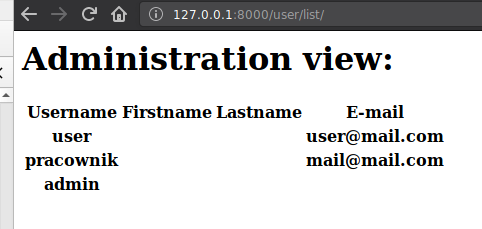
\includegraphics[scale=0.7]{img/16.png}
		\caption{Informacje o userze dla administratora}
	\end{figure}
	\begin{figure}[H]
		\centering
		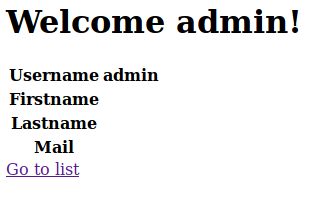
\includegraphics[scale=0.7]{img/15.png}
		\caption{Lista użytkowników}
	\end{figure}
	\subsection{Sprawdzenie listy faktur i pobranie interesujących}
	Z panelu głównego wybieramy 'Invoices'.
	\begin{figure}[H]
		\centering
		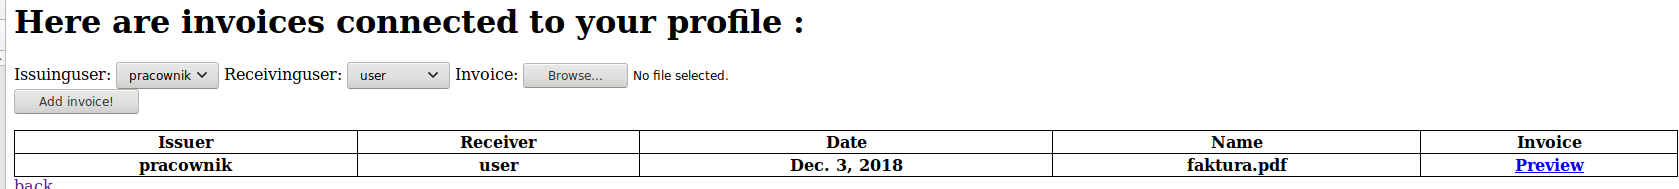
\includegraphics[scale=0.3]{img/8.png}
		\caption{Lista faktur}
	\end{figure}
	Widzimy wszystkie adresowane do nas faktury. Po wybraniu 'Preview' możemy pobrać wybraną.
	
	\subsection{Wystawienie nowych faktur (dla pracownika)}
	Z panelu głównego wybieramy 'Invoices'.
	\begin{figure}[H]
		\centering
		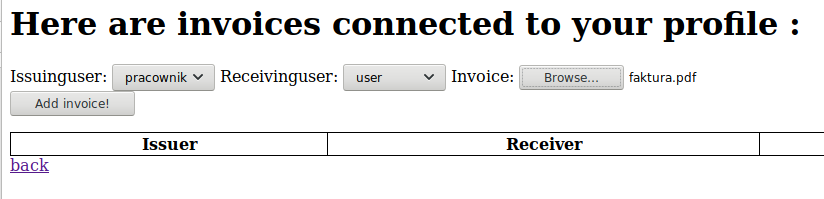
\includegraphics[scale=0.5]{img/7.png}
		\caption{Pusta lista faktur, podczas wypełniania}
	\end{figure}
	Należy wypełnić pola, aby dodać fakturę. Po dodaniu faktury automatycznie tworzona jest notyfikacja.
	\begin{figure}[H]
		\centering
		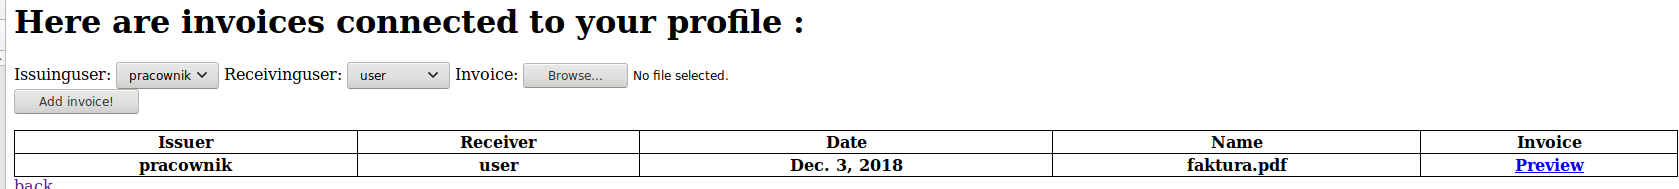
\includegraphics[scale=0.3]{img/8.png}
		\caption{Dodana faktura}
	\end{figure}
	\subsection{Przeglądanie forum}
	Po wybraniu 'Forum' ze strony głównej, możemy przeglądać kategorie, oraz dodawać nowe.
	\begin{figure}[H]
		\centering
		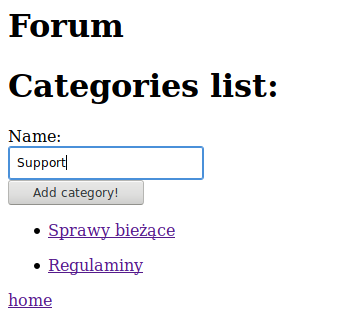
\includegraphics[scale=0.7]{img/10.png}
		\caption{Widok kategorii}
	\end{figure}
	Tak samo po wejściu w kategorię widzimy poszczególne wątki.
	\begin{figure}[H]
		\centering
		
\includegraphics[scale=0.7]{img/11.png}
		\caption{Widok wątków}
	\end{figure}
	\subsection{Dodawanie nowych wątków i postów}
	We właściwym widoku dodajemy nowy wątek (automatycznie jest generowany pusty).
	\begin{figure}[H]
		\centering
		
\includegraphics[scale=0.7]{img/11.png}
		\caption{Widok wątków}
	\end{figure}
	Potem wchodzimy w niego i możemy już swobodnie dodawać posty.
	\begin{figure}[H]
		\centering
		
\includegraphics[scale=0.5]{img/13.png}
		\caption{Widok pojedyńczego wątku}
	\end{figure}
	Dodanie postu generuje notyfikację.
	\begin{figure}[H]
		\centering
		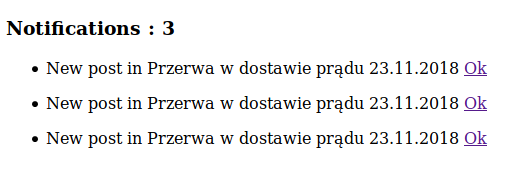
\includegraphics[scale=0.7]{img/14.png}
		\caption{Lista notyfikacji}
	\end{figure}
	
	\section{Opis aplikacji od strony programistycznej}
	\subsection{Architektura aplikacji}
	W celu utrzymania prostoty projektu, użyto standardowego dla Django wzorca model-template-view, który jest pokrewny z MVC. Dzięki temu mamy wydzieloną część bazodanową, ukrytą za modelem, szablony poszczególnych podstron oraz obsługę widoków. Każdy z tych elementów zostanie przedstawiony poniżej.
	
	\subsection{Bezpieczeństwo}
	Podstrony z ograniczonym dostępem dla danych użytkowników są dodatkowo sprawdzane podczas wczytywania (pierwsza linia):
	\begin{figure}[H]
		\centering
		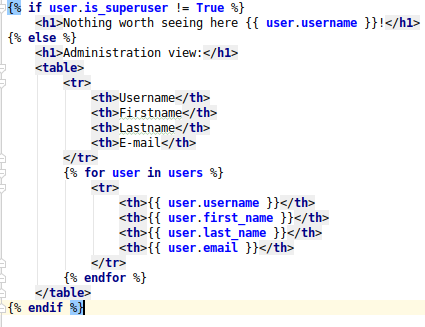
\includegraphics[scale=0.7]{img/c_template_security.png}
		\caption{Zabezpieczenie szablonu przed niepoprawnym wyświetleniem}
	\end{figure}
	Oprócz tego wdrożono podstawową autoryzację uniemożliwiającą dostęp do stron bez zalogowania.
	
	\subsection{Diagram związków encji}
	Został on przedstawiony w notacji Martina (kruczej stopki).
	
	\begin{figure}[H]
		\centering
		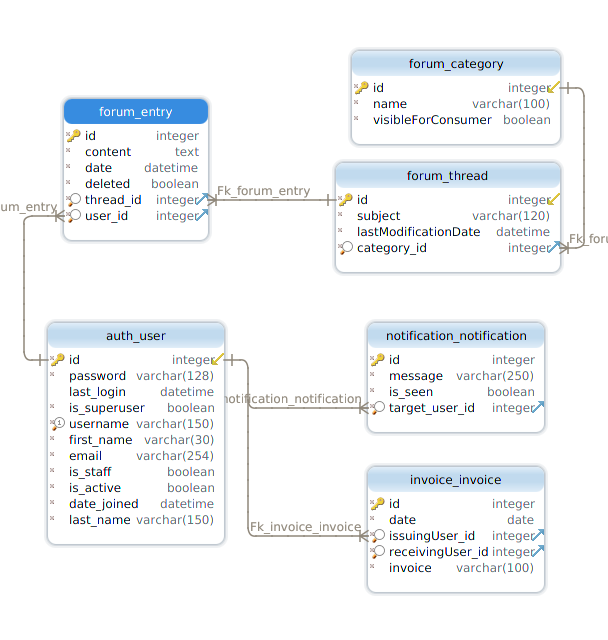
\includegraphics[scale=0.8]{img/sqlite.png}
		\caption{Diagram związków encji}
		\label{}
	\end{figure}
	
	\subsection{Mapowanie ORM}
	Baza danych jest tworzona na podstawie zdefiniowanych klas, dla przykładu forum:
	\begin{figure}[H]
		\centering
		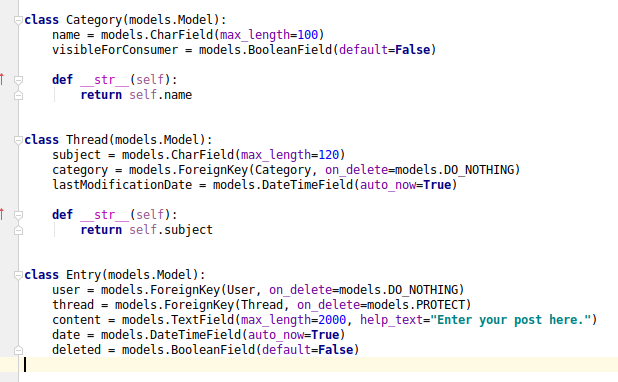
\includegraphics[scale=0.7]{img/c_forum_model.png}
		\caption{Model ORM forum}
	\end{figure}
	\newpage
	\subsection{Widoki}
	Widoki są podstawą jeżeli mowa o komunikacji z bazą danych i użytkownikiem. Udostępniają poszczególne metody, które reagują odpowiednio zależnie od odebranych danych.
	\begin{figure}[H]
		\centering
		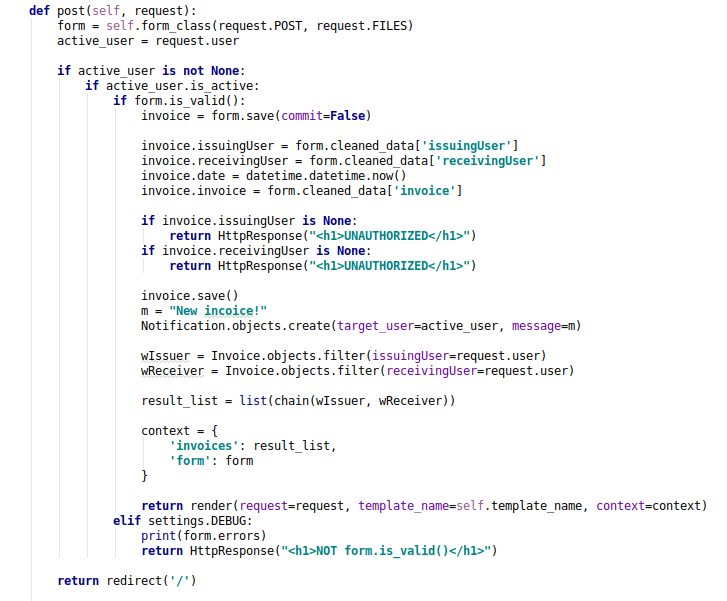
\includegraphics[scale=0.7]{img/c_invoice_post.png}
		\caption{Metoda post w invoice}
	\end{figure}
	\begin{figure}[H]
		\centering
		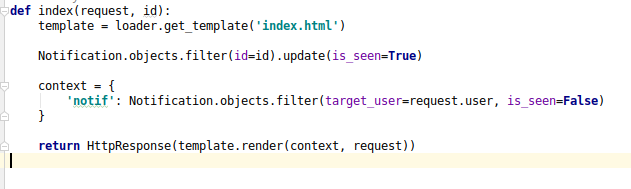
\includegraphics[scale=0.7]{img/c_notify_view.png}
		\caption{Realizacja chowania notyfikacji}
	\end{figure}
	\begin{figure}[H]
		\centering
		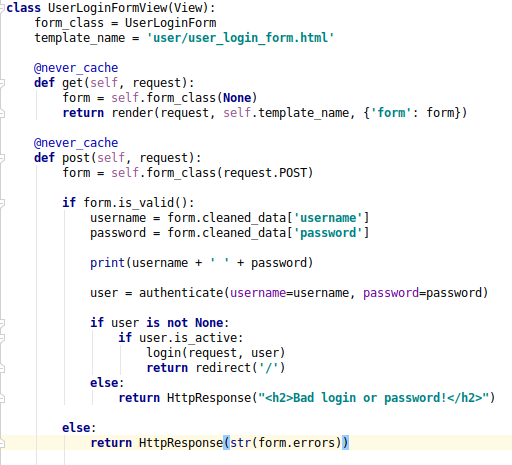
\includegraphics[scale=0.7]{img/c_user_login.png}
		\caption{Formularz logowania}
	\end{figure}
	\newpage
	\subsection{Szablony}
	Decydują o wyglądzie danych przekazanych przez widok, pozwalają na dynamiczne podejmowanie decyzji podczas ich tworzenia.
	\begin{figure}[H]
		\centering
		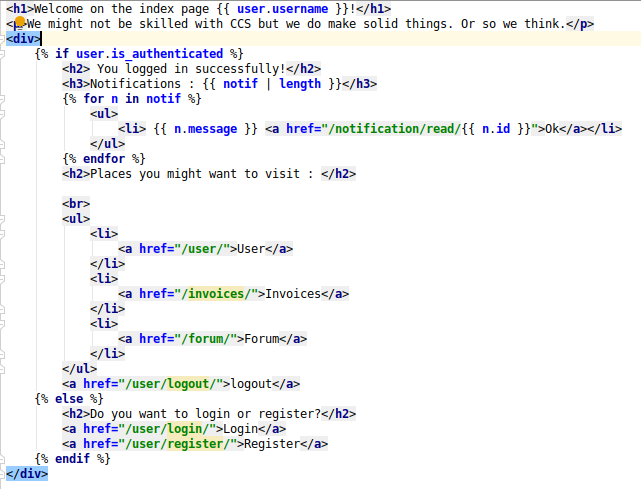
\includegraphics[scale=0.7]{img/c_template.png}
		\caption{Strona główna}
	\end{figure}
	\begin{figure}[H]
		\centering
		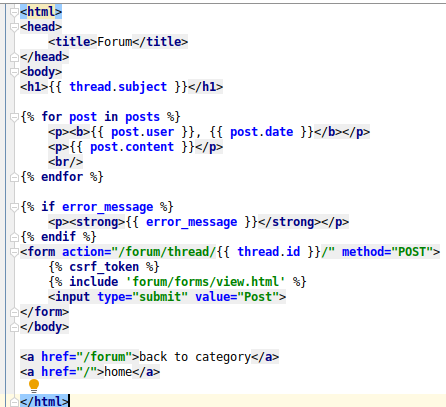
\includegraphics[scale=0.7]{img/c_forum_template.png}
		\caption{Forum - szablon konkretnego wątku}
	\end{figure}
	\newpage
	\subsection{Urls}
	Istnieją także wzorce do rozwiązywania adresów, na których opierają się widoki, oraz szablony:
	\begin{figure}[H]
		\centering
		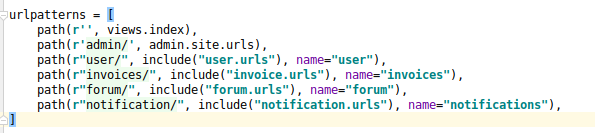
\includegraphics[scale=0.7]{img/c_urls.png}
		\caption{Podstawowe rozwiązywanie url-i}
	\end{figure}
	\begin{figure}[H]
		\centering
		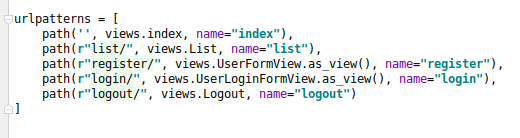
\includegraphics[scale=0.7]{img/c_user_urls.png}
		\caption{Dodatkowe wzorce dla logowania}
	\end{figure}
	
	\section{Instrukcja wdrożenia}
	Insturkcja obejmuje jedynie uruchomienie Django, ze względu na mnogość możliwych konfiguracji.
	
	Należy pobrać repozytorium na serwer:
	\begin{quote}
		git copy https://github.com/TheMesoria/RemoteDataBases.git
	\end{quote}
	Wymagany jest python3 oraz pip3. Tworzymy virtualenv:
	\begin{quote}pip3 install virtualenv\end{quote}
	\begin{quote}virtualenv venv\end{quote}
	\begin{quote}source venv/bin/activate\end{quote}
	Następnie instalujemy Django:
	\begin{quote}pip3 install django\end{quote}
	Możemy zweryfikować poprawność instalacji:
	\begin{quote}django-admin --version\end{quote}
	Przed uruchomieniem aplikacji należy dokonać migracji:
	\begin{quote}python3 manage.py makemigrations user invoice notification forum\end{quote}
	\begin{quote}python3 manage.py migrate\end{quote}
	Testowe uruchomienie serewera jest możliwe bezpośrednio z frameworka:
	\begin{quote}python manage.py runserver 80\end{quote}
	Właściwa konfiguracja serwera należy już do osoby wdrażającej aplikację na konkretny typ serwera.
	
	Dla bezpieczeństwa konieczna jest zmiana kluczy i wyłączenie trybu debugowania:
	\begin{figure}[H]
		\centering
		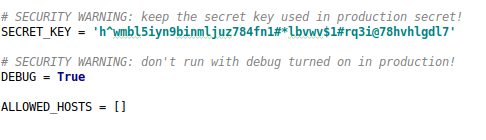
\includegraphics[scale=0.7]{img/c_security.png}
		\caption{Ważne opcje bezpieczeństwa}
	\end{figure}
	\newpage
	\section{Podsumowanie}
	Dzięki dokładnej analizie potrzeb klienta otrzymaliśmy kompletny zestaw wymagań, które powinny być spełnione. Umożliwiło to lepsze zaprojektowanie modularnego systemu, który można w prosty sposób zmieniać, gdy te wymagania ulegną modyfikacji. Następnie zaimplementowaliśmy niezbędne funkcjonalności oraz przeprowadziliśmy wdrożenie aplikacji.
	
	Finalnie, system wspiera firmę w przekazywaniu faktur klientom. Do informowania klienta jest wykorzystywany także system powiadomień. Przekazuje on informacje o nowych postach na forum, które jest ostatnią funkcjonalnością, jaka została wdrożona. Całość ma za zadanie usprawnić komunikację między firmą kupującą nasze rozwiązanie, a jej klientami.
	
	\section{Literatura}
	\begin{itemize}
		\item Wykład z Internetowych Baz Danych: \url{http://roman.ptak.staff.iiar.pwr.wroc.pl/}
		\item Dokumentacja Pythona 3.6: \url{https://docs.python.org/3.6/}
		\item Dokumentacja Django 2.1.2: \url{https://docs.djangoproject.com/en/2.1/contents/}
		\item Dokumentacja HTML5: \url{https://www.w3.org/TR/html5/}
	\end{itemize}
	
\end{document}